\graphicspath{{chapters/20/images/}}
\chapter{Advanced methods}

\section{Adiabatic dynamics}
In the free energy adiabatic dynamics the idea is to obtain the free energy hypersurface as a function of some reaction coordinates.
Let's assume the reaction coordinates $n<3N$ reaction coordinates with generalized coordinates $q_\alpha$: the interest is in the free energy hypersurface $A(q_1, \dots, q_n)$.
The partition function is defined, in the case of the canonica ensemble, as:

$$Q(N, V, T) = C_N\int d^N\vec{p}d^N\vec{r}e^{-\beta\biggl[\sum\limits_{i=1}^N\frac{\vec{p}_i^2}{2m_i}+U(\vec{r}_1, \dots, \vec{r}_N)\biggr]}$$

Transformation to generalized coordinates $q_\alpha = f_\alpha(\vec{r}_1, \dots, \vec{r}_n)$ only for the configurational part, leaving momenta unchanged:

$$Q(N, V, T) = C_n\int d^N\vec{p}d^{3N}qe^{-\beta\biggl[\sum\limits_{i=1}^N\frac{\vec{p}_i^2}{2m_i} + \tilde{V}(q_1, \dots, q_{3N}, \beta)\biggr]}$$

Where, considering the Jacobian of the transformation:

$$\tilde{V}(q_1, \dots, q_{3N}, \beta) = \tilde{U}(q_1, \dots, q_{3N}) - kT\ln J(q_1, \dots, q_{3N})$$

This is a function of all of the $3N$ coordinates.
This term looks like a potential in term with the generalized coordinates and the Jacobian.
In this term the potential is temperature dependent.
This is because $\tilde{V}$ has $\beta$ as a temperature parameters.
Using the Hamiltonian in the transformation during the simulation the canonical distribution is being sampled.
So consider the temperature dependent potential included into this fake Hamiltonian:

$$\tilde{\mathcal{H}}(q, \vec{p}, \beta) = \sum\limits_{i=1}^N\frac{\vec{p}_i^2}{2m_i}+\tilde{V}(q_1, \dots, q_{3N}, \beta) = \sum\limits_{i=1}^N\frac{\vec{p}_i^2}{2m_i}+\tilde{U}(q_1, \dots, q_{3N})-kT\ln J(q_1, \dots, q_{3N})$$

To conjugate the momenta to the velocities they need to be renamed.
This is not the original Hamiltonian but can be used as a Hamiltonian.
Renaming the momenta:

$$\tilde{H}(q, p, \beta) = \sum\limits_{\alpha=1}^{3N}\frac{p_\alpha^2}{2m'_\alpha}+ \tilde{V}(q_1, \dots, q_{3N}, \beta)$$

Where $m'_\alpha$ is a fictitious mass defined during the simulation.
As in adiabatic free energy dynamics the first $n$ variables are thermostatted as a temperature $T_q\gg T$ with their masses increased so to adiabatically decouple them from the others.
So the system should be have enough time to equilibrate for each variable.

	\subsection{TAMD}
	The previous idea can be implemented as TAMD (temperature accelerated molecular dynamics).
	Using the Hamiltonian with the renamed momenta:

	$$\tilde{H}(q, p, \beta) = \sum\limits_{\alpha=1}^{3N}\frac{p_\alpha^2}{2m'_\alpha} + \tilde{V}(q_1, \dots, q_{3N}, \beta)$$

	So that the differential equation to update positions:

	$$\dot{q}_\alpha = \frac{p_\alpha}{m'_\alpha}$$

	And momenta, where they are coupled with the thermostat variables needed to couple them to the Nos\`e-Hoover chain:

	$$\dot{p}_\alpha = -\frac{\partial\tilde{V}}{\partial q_\alpha} - \frac{p_{\eta_1}}{Q_1}p_\alpha\quad \alpha= 1, \dots, n\qquad\dot{p}_\alpha = -\frac{\partial\tilde{V}}{\partial q_\alpha}-\frac{p_{\eta_e}}{Q_2}p_\alpha\quad \alpha = n_1, \dots, 3N$$

	Then the variable for the thermostats:

	$$\dot{\eta}_j = \frac{p_{\eta_j}}{Q_j}$$

	Then the thermostat variable for the first $n$ generalized coordinates with $T_q$ higher tan $T$, while the other are coupled for the temperature $T$.

	$$\dot{p}_{\eta_1} = \sum\limits_{\alpha=1}^n\frac{p_\alpha^2}{2m'_\alpha}-nkT_q\qquad \dot{p}_{\epsilon_2} = \sum\limits_{\alpha=n+1}^{3N}\frac{p_\alpha^2}{2m'_\alpha}-(3N-n)kT$$

	It is possible to show that $A(q_1, \dots, q_n) = -kT_q\ln P_{adb}(q_1, \dots, q_n) + const$.
	So the free energy profile obtained by reconstructing the probability distribution for these $n$ generalized coordinate is equal to the one obtained for the energy profile at temperature $T$ in which the interest is in.
	An example can be seen in \ref{fig:tamd}, where it can be seen how the free energy profile using the bare potential is difficult to reconstruct the true analytical free energy.
	The others refers to TAMD and it can be seen how the mass associated to the reaction coordinate is much more the free energy profile is reconstructed well.
	This is because only in this case the system has enough time to explore the space at that value.

	\begin{figure}[H]
		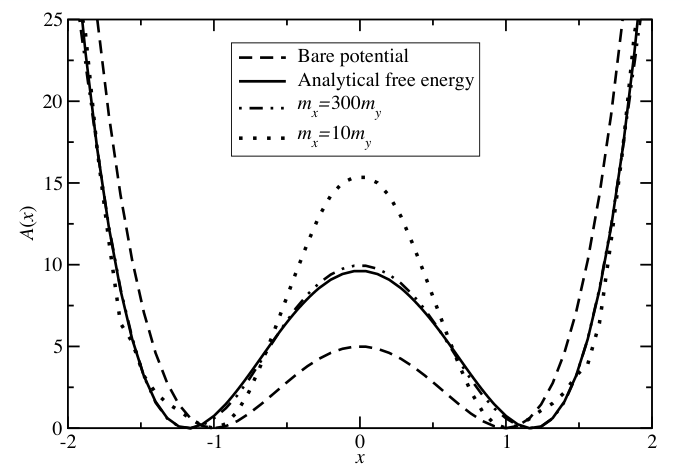
\includegraphics[width=\textwidth]{tamd}
		\caption{TAMD}
		\label{fig:tamd}
	\end{figure}

\section{Metadynamics}
The objective is to reconstruct a probability for a set of reaction coordinates $s_1, \dots, s_n$ and the objective is to obtain the ensemble average for a function of reaction coordinates:

$$P(s_1, \dots, s_n) = \biggl\langle\prod\limits_{\alpha=1}^n\delta(f_\alpha(\vec{r}_1, \dots, \vec{r}_N)-s_\alpha)\biggr\rangle$$

Replacing phase space average with a time average over a trajectory.
This can be done only if the trajectory is ergodic:

$$P(s_1, \dots, s_n) = \lim\limits_{\mathcal{T}\rightarrow\infty}\frac{1}{\mathcal{T}}\int_0^{\mathcal{T}} dt\prod\limits_{\alpha=1}^n\delta(f_\alpha(\vec{r}_1, \dots, \vec{r}_N)-s_\alpha)$$

Where $\mathcal{T}$ is time.
However considering the following property of the delta function:

$$\delta(x-\alpha) = \lim\limits_{\sigma\rightarrow 0}\frac{1}{\sqrt{2\pi\sigma^2}}e^{-\frac{(x-\alpha)^2}{2\sigma^2}}$$

So adding this property to the probability distribution:

$$P(s_1, \dots, s_n) = \lim\limits_{\mathcal{T}\rightarrow\infty}\lim\limits_{\Delta s\rightarrow 0}\frac{1}{\mathcal{T}}\frac{1}{\sqrt{2\pi\Delta s^2}}\int_0^{\mathcal{T}}dt\prod\limits_{\alpha=1}^ne^{-\frac{(s_\alpha-f_\alpha(\vec{r}_1(t), \dots, \vec{r}_N(t)))^2}{2\Delta s^2}}$$

This looks like adding to the probability a factor similar to the Boltzmann factor and related to it because it looks like a Gaussian.
It looks like a Gaussian is added every time a value for a reaction coordinate $\alpha$ is visited so that the system will be forced to go somewhere else.
Building up these Gaussian potential they can be used as a bias potential:

$$U_G(\vec{r}_1, \dots, \vec{r}_N, t) = W\sum\limits_{t - \tau_G, 2\tau_G, \dots}e^{-\sum\limits_{\alpha=1}^n\frac{(f_\alpha(\vec{r})-f_\alpha(\vec{r}_G(t)))^2}{2\Delta s^2}}$$

This Gaussian potential is added at every $\tau_G$, the conformation already visited will be less favoured and the system will go somewhere else.
Taking all the Gaussian added this amount to summing over all the Gaussian it is the negative of the free-energy profiles, so keeping track of the added Gaussians, their sum is minus the free energy profile.
This is done only when the free diffusion of the system is observed, meaning that the algorithm has reached convergence.
Judging convergence is not easy for metadynamics.
In principle it is continued until free diffusion is observed for a number of times.
Another issue is that every time energy is being added to the system, which might cause problem.
For example in a membrane it would cause membrane disruption.

\section{Transition path ensemble}
In many situations the interest is in reconstructing a path for a transition going from state $A$ to state $B$.
Assume that by some method a pathway to go from state $A$ to state $B$ is obtained.

\begin{figure}[H]
	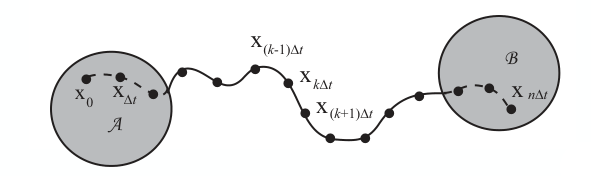
\includegraphics[width=\textwidth]{transition-path-ensemble}
	\caption{Transition path ensemble}
	\label{fig:transition-path-ensemble}
\end{figure}

To obtain the most probable path the transition path ensemble has to be introduced.
In order to reconstruct one point of the pathway in molecular dynamics Trotter factorization is applied:

$$x_{(k+1)\Delta t} = e^{iL_2\frac{\Delta t}{2}}e^{iL_1\Delta t}e^{iL_2\frac{\Delta t}{2}}x_{k\Delta t}\equiv\phi_{\Delta t}(x_{k\Delta t})$$

Considering in term of Monte Carlo moves instead:

$$T(x_{(k+1)\Delta t}|x_{k\Delta t}) = \delta(x_{(k+1)\Delta t}-\phi_{\Delta t}(x_{k_{\Delta t}}))$$

Assigning a weight to a single trajectory:

$$\mathcal{P}[X(\mathcal{T})] = f(x_0)\prod\limits_{k=0}^{n-1}T(x_{(k+1)\Delta t}|x_{k\Delta t})\qquad f(x_0) = \frac{e^{-\beta\mathcal{H}(x_0)}}{Q(N, V, T)}$$

This probability is given by starting from starting in $x_0$, which depends on the canonical distribution.
So $\mathcal{P}$ is the probability associated with a single trajectory.

$$\mathcal{P}[X(\mathcal{T})] = f(x_0)\prod\limits_{k=0}^{n-1}T(x_{(k+1)\Delta t}|x_{k\Delta t})$$


Defining the probability of a path $X$ going from $A$ to $B$ multiplies the probability associated for the path $X$ multiplied by $h_A$ and $h_B$, meaning that the starting point should be in the basin of state $A$ and the final point in the basin of state $B$, they are either $0$ or $1$.

$$\mathcal{P}_{AB}[X(\mathcal{T})] = \frac{1}{\mathcal{F}_{AB}(\mathcal{T})}h_A(x_0)\mathcal{P}[X(\mathcal{T})]h_B(x_{n\Delta t})$$

And $\mathcal{F}_{AB}$ is a normalization constant.

$$F_{AB}(\mathcal{T}) = \int dx_0\cdots dx_{n\Delta t}h_a(x_0)\mathcal{P}[X(\mathcal{T})]h_B(x_{n\Delta t})$$

For deterministic molecular dynamics trajectories:

\begin{align*}
	\mathcal{F}_{AB}(\mathcal{T}) &= \int dx_0\cdots dx_{n\Delta t}h_A(x_0)f(x_0)\prod\limits_{k=1}^{n-1}\delta(x_{(k+1)\Delta t}-\phi_{\Delta t}(x_{k\Delta t}))h_B(x_{n\Delta t}) = \\
																&=\int dx_0h_A(x_0)f(x_0)h_B(x_{n\Delta t}(x_0))
\end{align*}

	\subsection{Transition path sampling}
	Following the same method in Monte Carlo methods and Metropolis algorithm, introduce $\mathcal{R}_{AB}[X(\mathcal{T})|Y(\mathcal{T})]$, the conditional probability to generate a trajectory $X(\mathcal{T})$ starting from $Y(\mathcal{T})$.
	Considering the detailed balance condition:

	$$\mathcal{R}_{AB}[X(\mathcal{T})|Y(\mathcal{T})]\mathcal{P}_{AB}[Y(\mathcal{T})] = \mathcal{R}_{AB}[Y(\mathcal{T})|X(\mathcal{T})]\mathcal{P}_{AB}[X(\mathcal{T})]$$

	Splitting the conditional probabilities in two: one of generating the move and the other the probability to accept the move.

	$$\mathcal{R}_{AB}[X(\mathcal{T})|Y(\mathcal{T})] = \Lambda_{AB}[X(\mathcal{T})|Y(\mathcal{T})]\mathcal{T}_{AB}[X(\mathcal{T})|Y(\mathcal{T})]$$

	So now the acceptance probability can be written as:

	$$\Lambda_{AB}[X(\mathcal{T})|Y(\mathcal{T})] = \min\biggl[1, \frac{\mathcal{T}_{AB}[Y(\mathcal{T})|X(\mathcal{T})]\mathcal{P}_{AB}[X(\mathcal{T})]}{\mathcal{T}_{AB}[X(\mathcal{T})|Y(\mathcal{T})]\mathcal{P}_{AB}[Y(\mathcal{T})]}\biggr]$$

	In order to generate a move from $Y$ to $X$, it is assumed that $Y[\mathcal{T}]$ is a proper trajectory from $A$ to $B$, hence $h_A(y_0) = 1$ and $h_b(y_{n\Delta t}) = 1$.
	This means that the trajectory starts at $A$ and ends at $B$.
	Now a shooting move is performed: assuming that all the trajectories $Y$ start from state $A$ and end up in state $B$, then the only thing to check is the fact that the new trajectory starts at state $A$ and ends in state $B$:

	$$\Lambda_{AB}[X(\mathcal{T})|Y(\mathcal{T})] = h_A(x_0)h_B(x_{n\Delta t})\min\biggl[1, \frac{\mathcal{T}_{AB}[Y(\mathcal{T})|X(\mathcal{T})]\mathcal{P}_{AB}[X(\mathcal{T})]}{\mathcal{T}_{AB}[X(\mathcal{T})|Y(\mathcal{T})]\mathcal{P}_{AB}[Y(\mathcal{T})]}\biggr]$$

	\begin{figure}[H]
		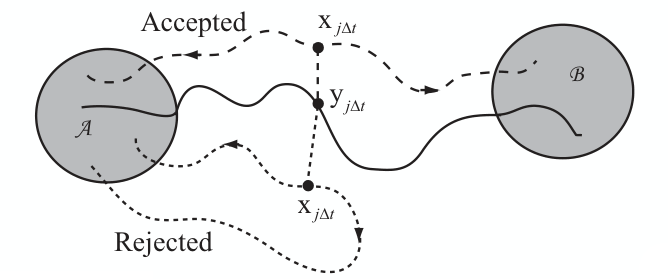
\includegraphics[width=\textwidth]{transition-path-sampling}
		\caption{Shooting move}
		\label{fig:shooting-move}
	\end{figure}

	Assuming that $Y$ is a given trajectory and starting from a random point $y_{i\Delta t}$ in $Y$, starting from the point the momenta are regenerated so there is a new position in the system $x_{j\Delta t}$.
	With this coordinate and momenta it is integrated forward and backward in time.
	Now if integrating backward it is ended in $A$ and forward in $B$.
	If integrating forward going back to state $A$, this move has to be rejected because this new path does not start from state $A$ and ends up in state $B$.
	In the first case the move is accepted.
	In this way new pathways starting from a reasonable one can be generated, exploring the ensemble associated to the transition paths.
	$\tau(x_{j\Delta t}|y_{j\Delta t})$ is the rule to generate the shooting point.
	So a randomly chosen $y$ point in time, so the coordinates are not changed but the momenta are generated from a Boltzmann distribution.
	Then the probability to generate path $X$ to path $Y$ it the product of the probability of generate the point, the probability to shoot forward in time and the probability to shoot backward in time:

	$$\mathcal{T}_{AB}[X(\mathcal{T})|Y(\mathcal{T})] = \tau(x_{j\Delta t}|y_{j\Delta t})\biggl[\prod\limits_{k=j}^{n-1}T(x_{(k+1)\Delta t}|x_{k\Delta t})\biggr]\biggl[\prod\limits_{k=1}^jT(x_{(k-1)\Delta t}|x_{k\Delta t})\biggr]$$

	Using a deterministic rule the $T$ becomes delta functions.
	Looking at the acceptance probability, making explicit the $\mathcal{T}$s it can be seen how the forward part can be simplified and assuming that $T$ is symmetric another simplification can be made.

	\begin{align*}
		\Lambda_{AB}[X(\mathcal{T})|Y(\mathcal{T})] &= h_A(x_0)h_B(x_{n\Delta t})\min\biggl[1, \frac{\mathcal{T}_{AB}[Y(\mathcal{T})|X(\mathcal{T})]\mathcal{P}_{AB}[X(\mathcal{T})]}{\mathcal{T}_{AB}[X(\mathcal{T})|Y(\mathcal{T})]\mathcal{P}_{AB}[Y(\mathcal{T})]}\biggr] = \\
																								&= h_A(x_0)h_B(x_{n\Delta t})\min\biggl[1, \frac{f(x_0)}{f(y_0)}\biggl(\prod\limits_{k=0}^{n-1}\frac{T(x_{(k+1)\Delta t}|x_{k\Delta t})}{T(y_{(k+1)\Delta t}|y_k\Delta t)}\biggr)\biggl(\frac{\tau(y_{i\Delta t}|x_{j\Delta t})}{\tau(x_{j\Delta t}|y_{j\Delta t})}\cdot\\
																								&\qquad\qquad\qquad\qquad\qquad\qquad\cdot\prod\limits_{k=j}^{n-1}\frac{T(y_{(k+1)\Delta t}|y_{k\Delta t})}{T(x_{(k+1)\Delta t}|x_{k\Delta t})}\prod\limits_{k=0}^{j-1}\frac{T(y_{k\Delta t}|y_{(k+1)\Delta t})}{T(x_{k\Delta t}|x_{(k+1)\Delta t})}\biggr)\biggr] = \\
																								&=h_A(x_0)h_B(x_{n\Delta t})\min\biggl[1, \frac{f(x_0)}{f(y_0)}\frac{\tau(y_{j\Delta t}|x_{j\Delta t})}{\tau(x_{j\Delta t}|y_{j\Delta t})}\prod\limits_{k=0}^{j-1}\frac{T(x_{(k+1)\Delta t}|x_{k\Delta t})}{T(y_{(k+1)\Delta t}|y_{k\Delta t})}\frac{T(y_{k\Delta t}|y_{(k+1)\Delta t})}{T(x_{k\Delta t}|x_{(k+1)\Delta t})}\biggr]=\\
																								& = h_A(x_0)h_B(x_{n\Delta t})\min\biggl[1, \frac{f(x_0)}{f(y_0)}\frac{\tau(y_{j\Delta t}|x_{j\Delta t})}{\tau(x_{j\Delta t}|y_{j\Delta t})}\biggr]
	\end{align*}

	For a symmetric move $\tau(y_{j\Delta t}|x_{j\Delta t}) = \tau(x_{j\Delta t}|y_{j\Delta t})$:

	$$\Lambda_{AB}[X(\mathcal{T})|T(\mathcal{T})] = h_A(x_0)h_B(x_{n\Delta t})\min\biggl[1, \frac{f(x_0)}{f(y_0)}\biggr]$$

	So now the probability of the acceptance is the rate of the Boltzmann factors.
	So now an algorithm is obtained so that the phase space displacement $\Delta = (0, \delta p)$ and the algorithm can be built up:

	\begin{enumerate}
		\item Choose an index $j$ randomly on the old trajectory $Y(\mathcal{T})$.
		\item Generate a random phase space displacement $\Delta$ in order to generate the new shooting point $x_{j\Delta t}$ from the old point $y_{j\Delta t}$.
		\item Integrate the equations of motion backwards in time from the shooting point to the initial condition $x_0$.
		\item If the initial condition $x_0$ is not in the phase space region $A$, reject the trial move.
		\item If $x_0\in A$ accept the move with probability $\min\biggl[1,\frac{f(x_0)}{f(y_0)}\biggr]$.
		\item Integrate the equations of motion forward in time to generate the final point $x_{n\Delta t}$.
		\item If $x_{n\Delta t}\in B$, accept the trial move, and reject it otherwise.
		\item If the path is rejected at steps $4, 5$ or $7$, then the old trajectory $Y(\mathcal{T})$ is counted again in the calculation of averages over the transition path ensemble
			Otherwise invert the momenta along the backward part of the path to yield a forward moving transition path $X(\mathcal{T})$ and replace the old trajectory $Y(\mathcal{T})$ by the new one $X(\mathcal{T})$
	\end{enumerate}

\section{The committor distribution}
The real with reaction coordinates is to find good reaction coordinates.
One way to check whether the reaction coordinate is a good one is the committor distribution.
The committor is the probability $p_B(\vec{r})$ that a trajectory initiated from a configruation $\vec{r}$ with velocities sampled from a Maxwell-Boltzmann distribution will arrive in state $B$ before state $A$.
By definition the committor distribution is $0$ in state $A$ and $1$ in state $B$.
Moreover isocommittor surfaces at different probabilities: all point in that surface will end up in state $B$ with the probability that defines it.
In the transition state the isocommittor surface is $p_B = \frac{1}{2}$.

\begin{figure}[H]
	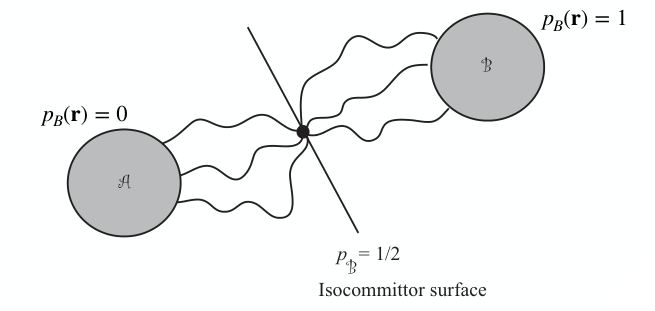
\includegraphics[width=\textwidth]{committor-distribution}
	\caption{The committor}
	\label{fig:committor-distribution}
\end{figure}

	\subsection{Histogram test}
	The committor $p_B(\vec{r})$ is an exact reaction coordinate for any system, but there is no analytic expression for it and obtaining it numerically is intractable.
	The reaction coordinate $q(\vec{r})$ is good when the isosurfaces $q(\vec{r}) = const$ approximates the isosurfaces $p_B(\vec{r})= const$ of the committor.
	The committor distribution is the probability that $p_B(\vec{r}) = p$ when $q(\vec{r}) = q^{\ddagger}$, the value of $q(\vec{r})$ at a presumptive transition state.
	Focussing on the transition state, the probability of the committor is:

	$$P(p) = \frac{C_N}{Q(N, V, T)}\int d^N\vec{p}\int_{q(\vec{r})=q^{\ddagger}}d^N\vec{r}e^{-\beta\mathcal{H}(\vec{r}, \vec{p})}\delta(p_B(\vec{r}_1, \dots, \vec{r}_N)-p)$$

	\subsection{Histogram test on $q_1(\vec{r}) = q^{\ddagger}$}
	To build up the histogram of the probabilities:

	\begin{enumerate}
		\item Fix the value $q_1(\vec{r}) = q^{\ddagger}$ at the transition state.
		\item Generate $M$ configurations for the other variables $q_2^{(k)}(\vec{r}), \dots, q_{3N}^{(k)}(\vec{r})$.
			Generate $M$ replicas for te system for which the reaction coordinate is fixed and the others are generated randomly.
		\item For each value of $k$, sample a set of initial velocities from a Maxwell-Boltzmann distribution.
		\item For each configuration $q^{\ddagger}, q_2^{(k)}(\vec{r}), \dots, q_{3N}^{(k)}(\vec{r})$, use each set of sampled velocities to initiate a trajectory and run it until the system ends up in A or B.
			Assign the trajectory the value $1$ if it ends up in state $B$ and $0$ if it ends up in state $A$.
			Take the average for this value of $k$ and store it as $p^{(k)}$.
		\item Repeat for all of the configurations sampled in step $2$ to generate $p^{(1)}, \dots, p^{(M)}$.
		\item Plot a histogram for $p^{(1)}, \dots, p^{(M)}$.
	\end{enumerate}

	If the histogram peaks at $0.5$ then the reaction coordinate was a good one.

	\begin{figure}[H]
		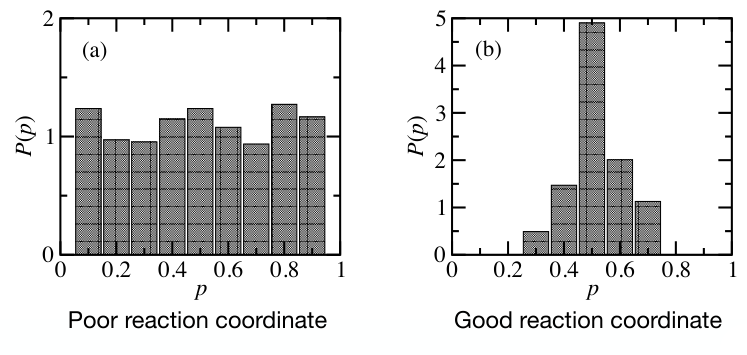
\includegraphics[width=\textwidth]{histogram-test}
		\caption{Histogram test example}
		\label{fig:histogram-test}
	\end{figure}
